\chapter{\agentj: Java Agents in NS2}
\label{agentj}

In this chapter, we present the design and implementation of the \agentj~
framework and show the various levels at which \agentj~interacts with other
software packages and implements its functionality. In the previous two 
chapters, Protolib and the PAI interface were described which form the 
building blocks for \agentj. This chapter shows how these have been integrated 
through extensive use of the java Java Native Interface (JNI). 

The first section provides an overview of the cooperating software 
components and the following section describes the core 
C++ and Java classes which have been used to implement these. Then,
for completeness, we present the Java version of the PAI interface, which
is at the core of this integration. Finally, we give a summary this integration by
providing a complete overview of the software component interactions and
the corresponding classes which implement the core behaviour of the system.  

Although, the understanding of the details of this chapter is not absolutely necessary 
for \agentj~users, it is highly recommended reading, as the details given here will
give a broad understanding of the \agentj~system and therefore, help a potential
user in understanding what s/he can and cannot do. 
 

\section{\agentj~Software Overview}
\label{agentj:nodeint}

Using \agentj, each C++ NS2 agent can (optionally) attach a Java agent. A 
Java Ns2 agent is a Java program that can be accessed through the 
standard \agentj~ interface, which allows it to receive commands in the 
same ways as C++ NS2 agents do. Thus, specifically, an \agentj~node is:

\emph{
\begin{quote}
A Java object that implements the \emph{AgentJObject} 
interface
\end{quote}
}

\vspace{0.2in}


\agentj~nodes can use any 3rd party Java application in order to
implement the behaviour they require. Further \agentj~nodes can
use the \agentj's PAI binding to access standard communication and 
timing classes in order to schedule events and discover and
communicate with other \agentj~nodes. In this fashion, complete
Java simulations can be built up using these simple primitives. 


For a Java application top become a \agentj~node, it only needs to 
implement a simple Java interface and so the overhead of converting a
Java applications into the \agentj~framework is minimal i.e. far easier 
that writing an Applet, for integration into another type of environment 
e.g. a Web browser.  However, for such \agentj~nodes to 
communicate with other nodes, they will need to interface with 
\agentj's re-implementations of the normal Java classes they would 
use. This normally involves replacing all occurances of 
\emph{java.net.} with \emph{pai.net.}.  We used precisely this procedure 
to integrate the  P2PS middleware, discussed in \cite{p2psx}.  

\index{P2PS}
\index{Applet}

In this section, we describe how the \agentj~framework 
has been integrated using JNI and the core C++ Protolib and PAI 
toolkits and Java classes. 

\index{PAI}
\index{Protolib}

\subsection{Creating \agentj~Nodes}
\label{agentj:creating}

\begin{figure}
\centering
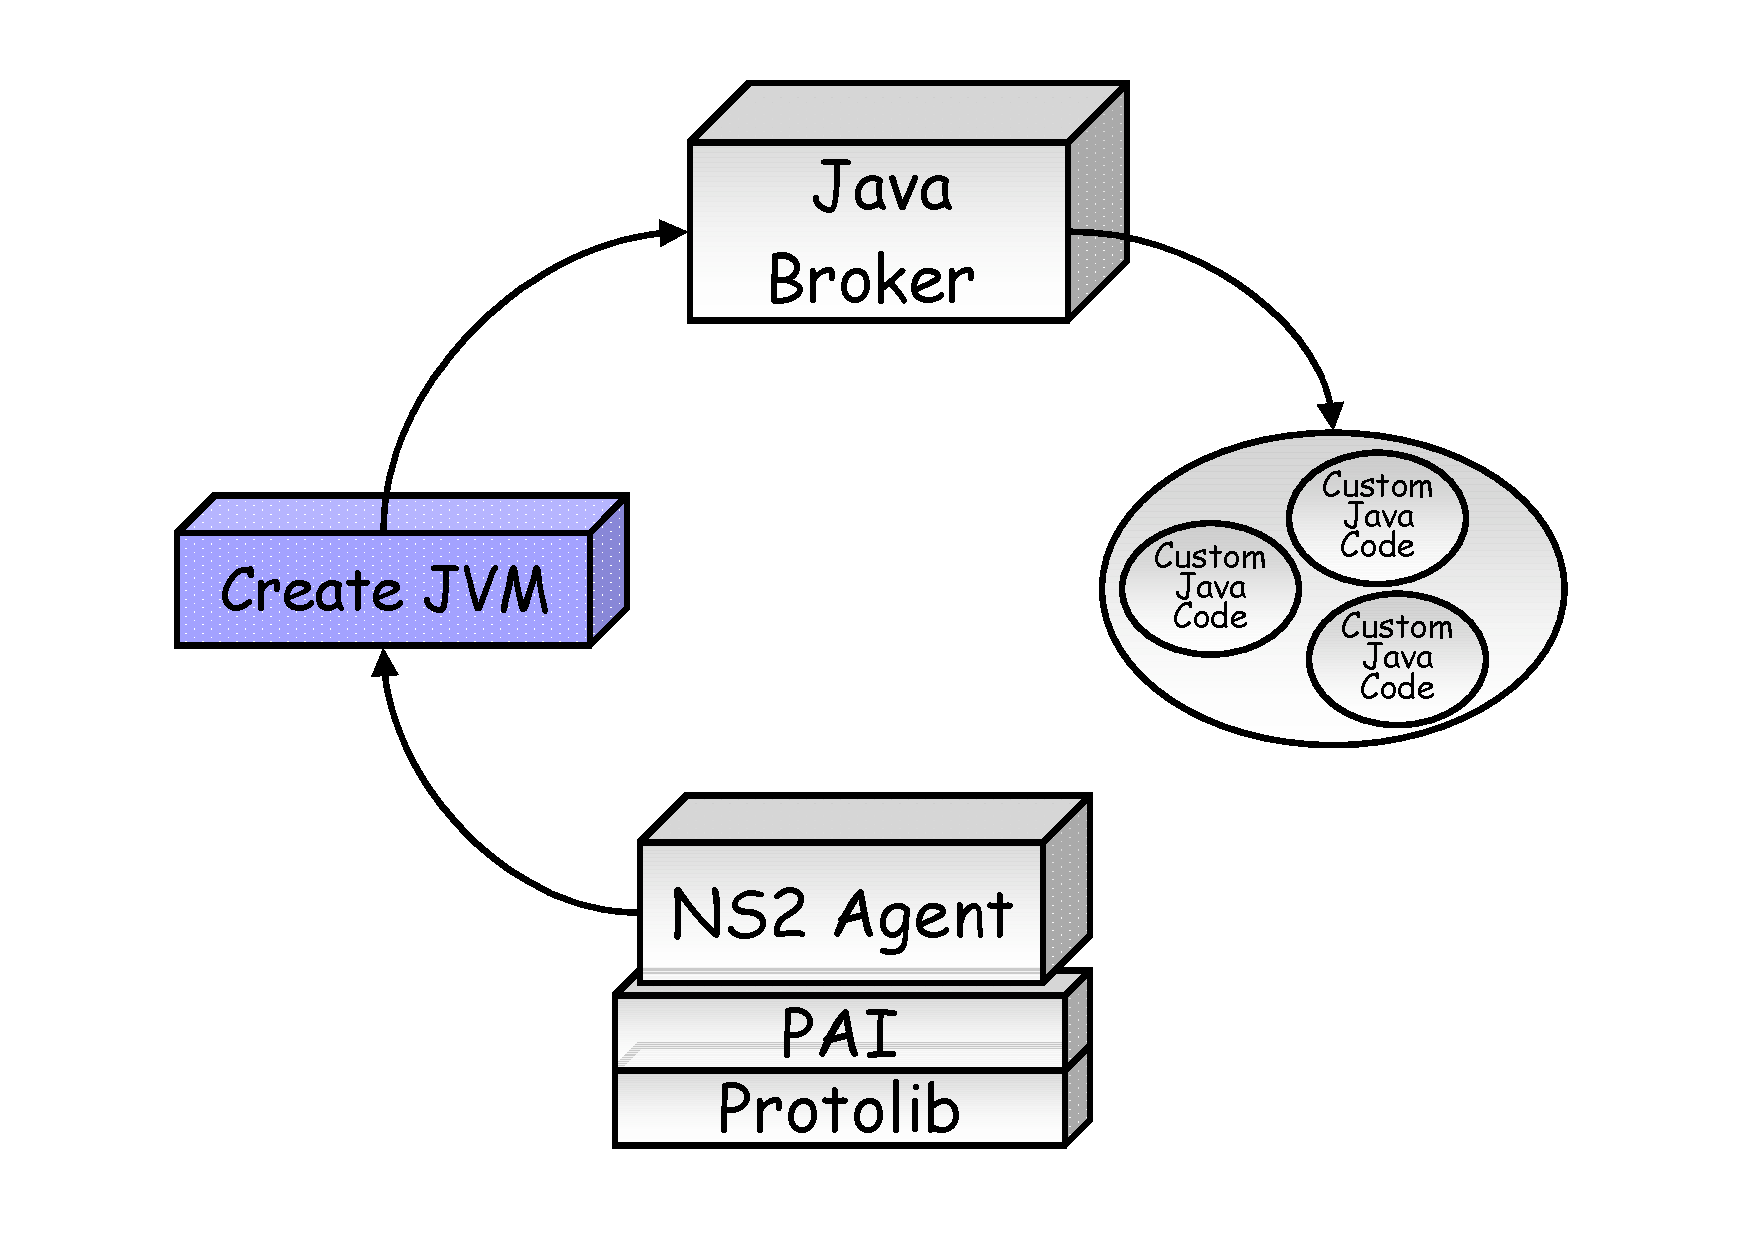
\includegraphics[scale=0.3]{images/agentjOverview}
\caption{\agentj~can attach any conforming Java object to an NS2 agent.} 
\label{agentj:fig:javaOverview}
\end{figure}

Figure \ref{agentj:fig:javaOverview} gives an overview of the software
architecture employed by \agentj~and shows how Java fits into
this picture.  Each NS2 \emph{agent} can attach a Java 
object (i.e. Java agent) by accessing a Java Virtual machine (JVM) 
and by requesting that an association be made within the Java domain
between the desired Java object and itself.  This request 
results in a Java Hashtable being populated with an item pair; with the 
C++ agent pointer representing the key and \agentj~Java object 
representing the object.   

\index{NS2}
\index{JNI}
\index{Java}
\index{JVM}

There could potentially be thousands of NS2 nodes and each one 
might want to instantiate and use a Java object.  Therefore serious 
scalability issues can be encountered if this interaction is not 
slimline enough. In \agentj, the C++ JVM helper class (C2JBroker) therefore
only allows \textbf{ONE} JVM to be  created no matter how many 
nodes exist in the simulations.  This JVM instantiates a singleton
the \emph{JavaBroker} class, which creates and manages the external 
Java objects. \emph{JavaBroker} contains functionality that can 
dynamically create a Java object from a textual representation of its
name (e.g. pai.examples.NS2.SimpleCommand). 

Once created such objects are added to a local Hashtable, which associates 
an NS2 agent's \emph{ID} with the associated object that has been created for this 
interaction.  The NS2 agent's \emph{ID} is actually its C++ pointer, which 
is reused later within the JNI binding (see below). Therefore, 
each NS2 node only instantiates the Java class it needs
rather than any other wrapping classes. This implementation therefore 
maps one-to-one between the C++ NS2 agent and its corresponding 
Java object and therefore keeps the memory allocation to an absolute 
minimum; that is, we do not create thousands of 
\emph{JavaBroker} objects, rather, we create one and have this act as
a central locator for all Java objects. 

The Java Hashtable is a static Class member (of JavaBroker.java, 
see section \ref{agentj:classes}) and therefore only one Hashtable exists for 
all Java agents.  When a node wishes to send a message to its attached 
Java object, it must first locate this object by searching this Hashtable using
the pointer to the C++ agent.  Once it has obtained a reference to the 
Java agent, it can forward the command to the object.  This searching
overhead is necessary for the issues discussed above in addressing
scalability. 

\subsection{Inter-\agentj~Communication}

Once an \agentj~node has been created and attached to its C++ 
counterpart, it can then use the supported \agentj~communication
and timing protocols in order to schedule events and 
communicate with other \agentj~nodes. \agentj~nodes do this
by using \textbf{standard Java interfaces} which have been 
re-implemented in order to bind to the simulation world within 
NS2. These implementations include:

\begin{itemize}
\item \textbf{UDP Transport:} DatagramSocket and Multicast Socket have been 
rebound to PAI and Protolib to work within NS2.
\item \textbf{TCP Transport:} under construction....
\item \textbf{Inet Support:} a number of the InetAddress methods have been
implemented to work within the NS2 context.
\item \textbf{Timing Libraries:} simple interfaces to timing functions have been 
implemented so that non realtime events (i.e. NS timing events) can be triggered 
at specific intervals during the simulation.
\end{itemize}

This functionality has been implemented by re-implementing the standard Java
interfaces to the networked Java counterparts of these functions. Therefore, in
order to use these within your Java program for example, you simply need to 
import the \emph{pai.net} versions of DatagramSocket and MulticastSocket
rather than the \emph{java.io} versions.


Figure \ref{agentj:fig:javaFullOverview} gives an overview of the lower layers
of this integration and provides a complete picture of how \agentj~uses Java 
within its implementation.  Here, the \agentj~nodes interface through the
Java PAI libraries by using a JNI binding to the C++ PAI and underlying 
Protolib toolkits. It is this software stack that describes the full integration.  
The standard Java interfaces described above merely provide convenient 
access to these libraries.

\begin{figure}
\centering
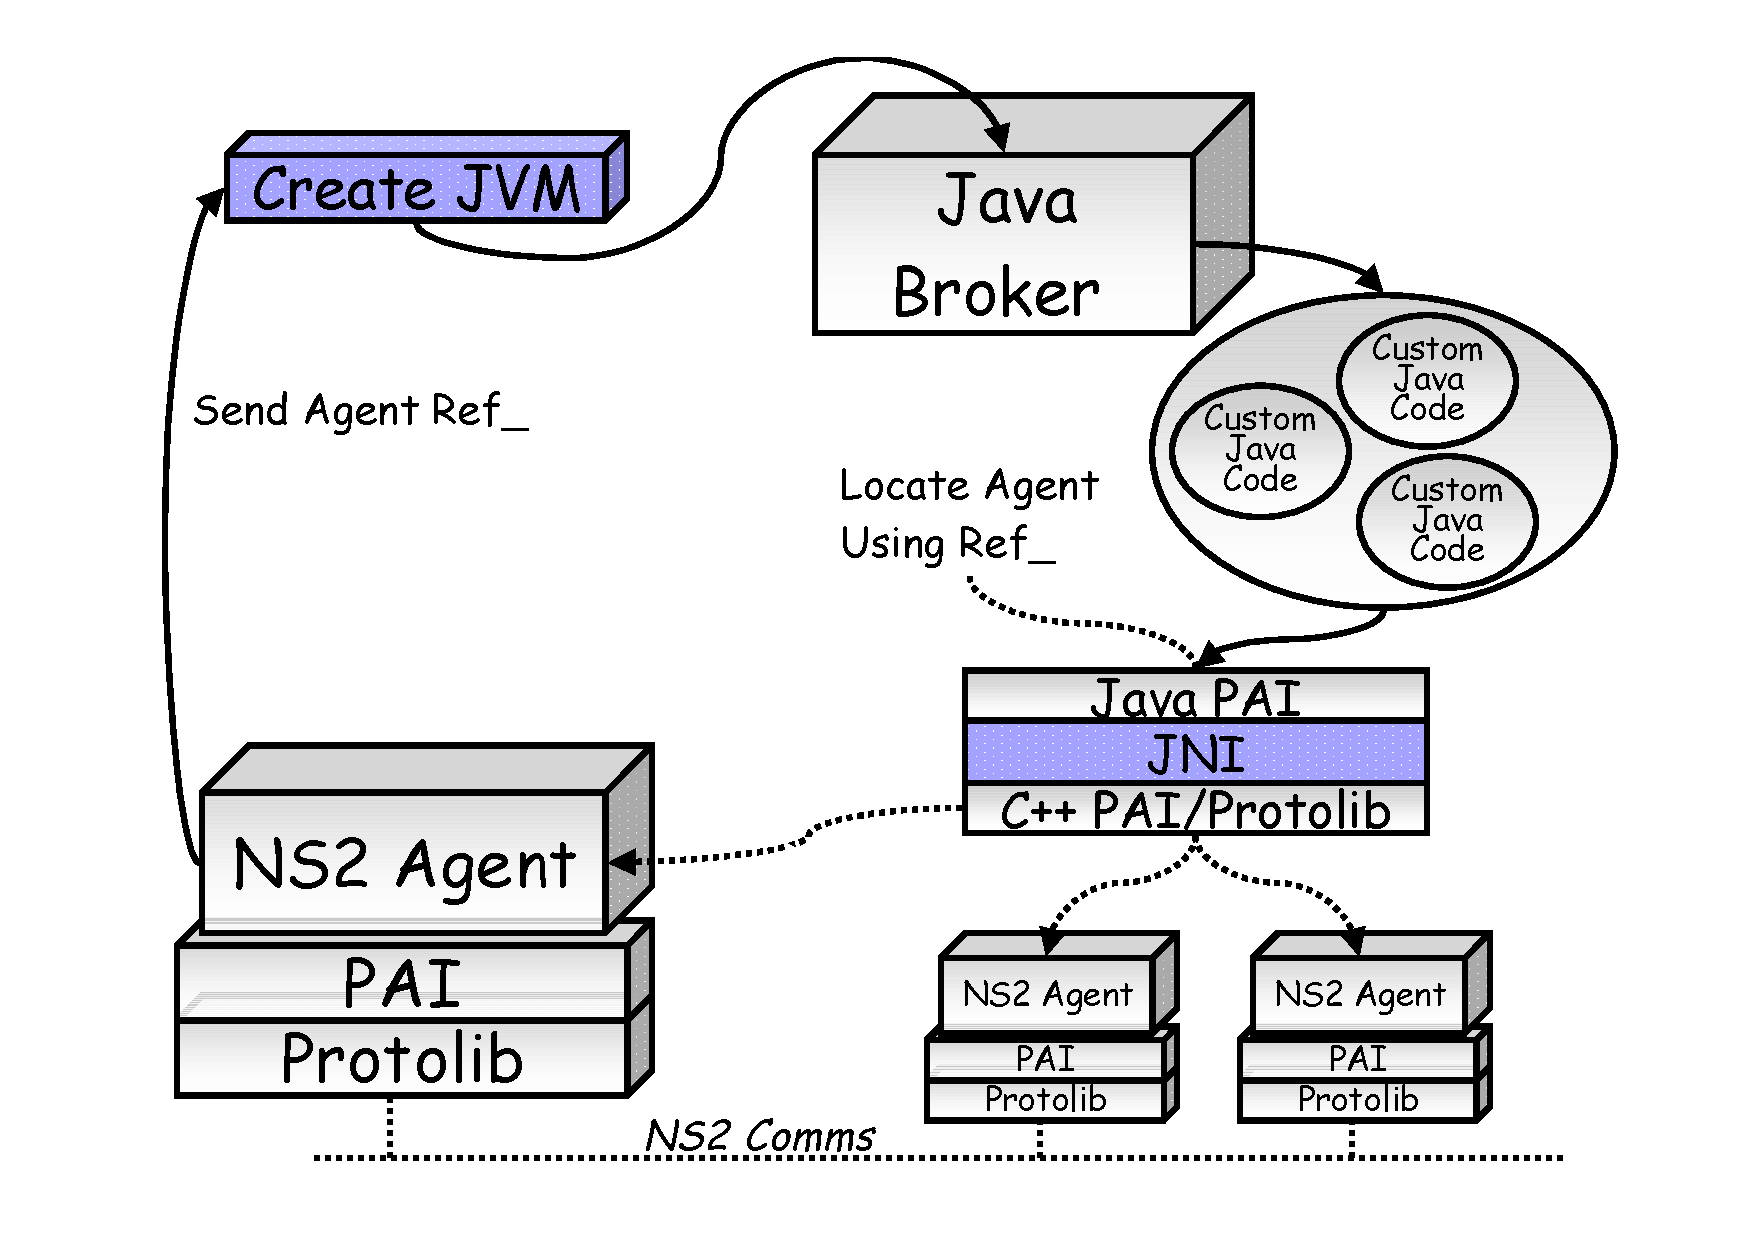
\includegraphics[scale=0.40]{images/agentjFullOverview}
\caption{An overview of the \agentj~software interaction between 
NS2, JNI, PAI and Protolib.} 
\label{agentj:fig:javaFullOverview}
\end{figure}

Therefore, an \agentj~node interacts with other \agentj~nodes 
by binding the standard Java interfaces to the PAI 
socket and timing classes within the JNI implementation, as 
indicated here. This integration allows \agentj~nodes to issue 
commands to send data between NS2 nodes and to set up callbacks
for timing events within NS2. 

For this implementation, a JNI interface is provided 
between the Java PAI interface and the corresponding C++ PAI 
interface that contains the necessary underlying 
functionality. Within this implementation, the \agentj~node's 
\emph{ID} is used along within the JNI binding to the 
PAI interface in order to re-associate the Java object within its 
C++ Ns2 agent when we return back to the C++ context.
In effect, what we are doing here is creating a JVM from C++,
then we are using JNI to re-enter C++. 

However, when we do 
this, JNI has no context and therefore we cannot use static
methods to obtain pointers to parts of the NS2 system. Therefore,
we have to transport these pointers manually through the JVM
so we can re-establish our context when we are back in the
C++ world. Specifically, the \agentj~node needs to be able to 
reference its corresponding C++ NS2 agent so it can invoke
the calls in the appropriate way. Otherwise, how would Protolib
know which node to send the data from?

\section{\agentj~Implementation}
\label{agentj:classes}

This section gives an overview of the classes used to implement
\agentj and describes the key classes that integrate the 
various components together.  There are many underlying 
classes which are not described here but this section
provides a good starting point for those interested in learning 
more about the integration.
 
\agentj~is made up of a collection of C++ and Java classes.  There
are many more C++ classes than Java as the majority of the
implementation is involved in binding between Protolib and
higher level implementations and Java interfaces. For example,
there are many housekeeping classes which provide lookup
tables for mapping between C++ callbacks and Java Listener 
interfaces and vice versa.  

Here, we provide descriptions for the key glue classes that tie the
various parts of the system together between the C++ Java 
classes. The underlying C++ code for PAI and the specifics
of these implementations are out of the scope of this chapter.  

\subsection{Organization of \agentj~Classes}

The \agentj~directorty tree is organized as if it was a Java application.  Therefore,
within this \agentj~directory, there is a classes directory (where all classes 
live), a lib directory (for JAR files plus shared libraries), a doc directory 
(containing this manual) and a src directory (for source files), amongst 
others. 

The src directory also is organized as if it was a Java application also (for the
Java parts AND the C++ parts).  I apologise in advance for this for those
C++ developers who follow different standards but I write C++ programs
as if they were Java and organize them as such! I believe however, that 
the overall structure is organized sensibly and due the the nature of this 
integration it is far easier to maintain a coherency between the Java and
C++ classes. 

\begin{figure}
\centering
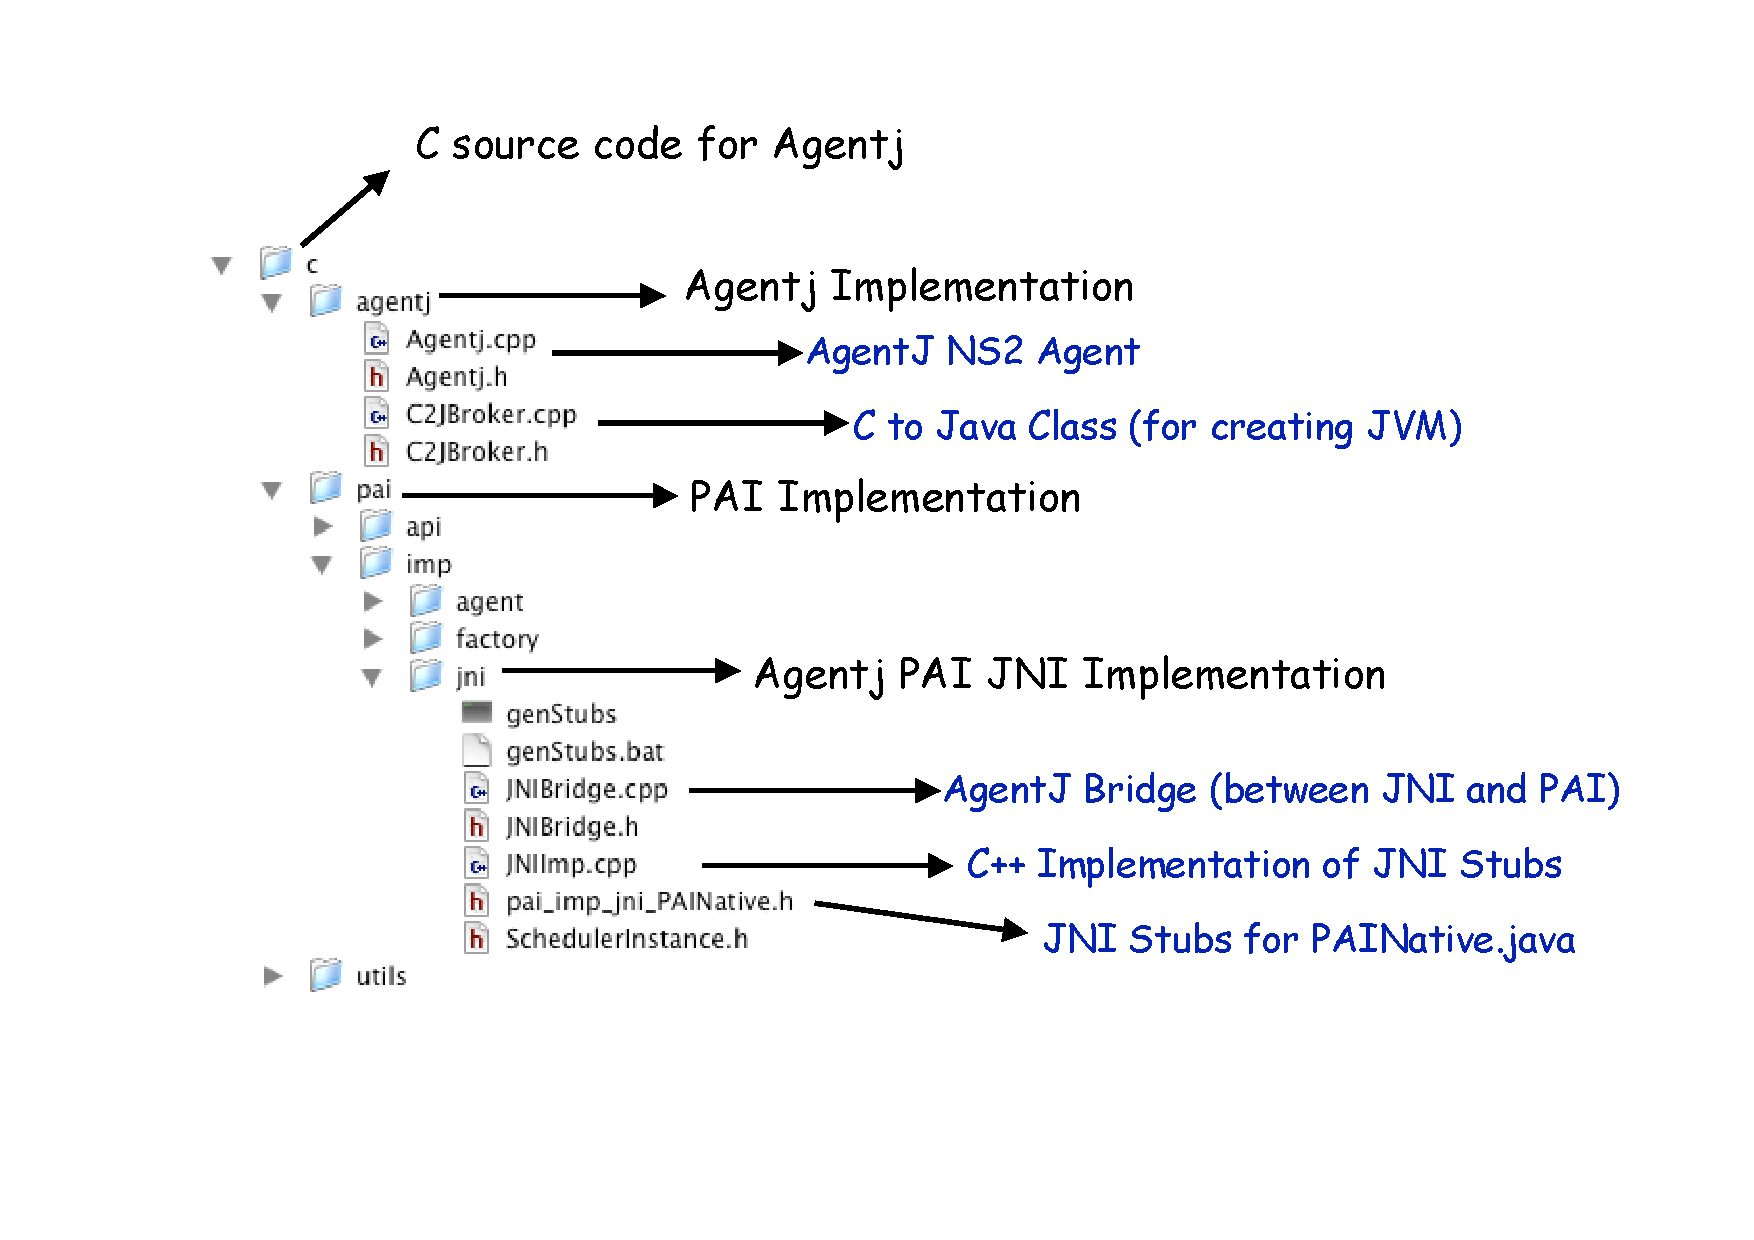
\includegraphics[scale=0.45]{images/agentjCClasses}
\caption{The C++ Classes within \agentj.} 
\label{agentj:fig:CClasses}
\end{figure}

At the top-level, there is a 'java' directory and a 'c' directory. These 
two directory structures are illustrated in Figures \ref{agentj:fig:CClasses} 
for C++ and \ref{agentj:fig:JavaClasses} for Java. At the next level,
both the Java and C source trees are split into two sub-directories,
one containing the classes specific to the implementation of
\agentj and the other to the supporting implementations of
PAI, as illustrated.

\begin{figure}
\centering
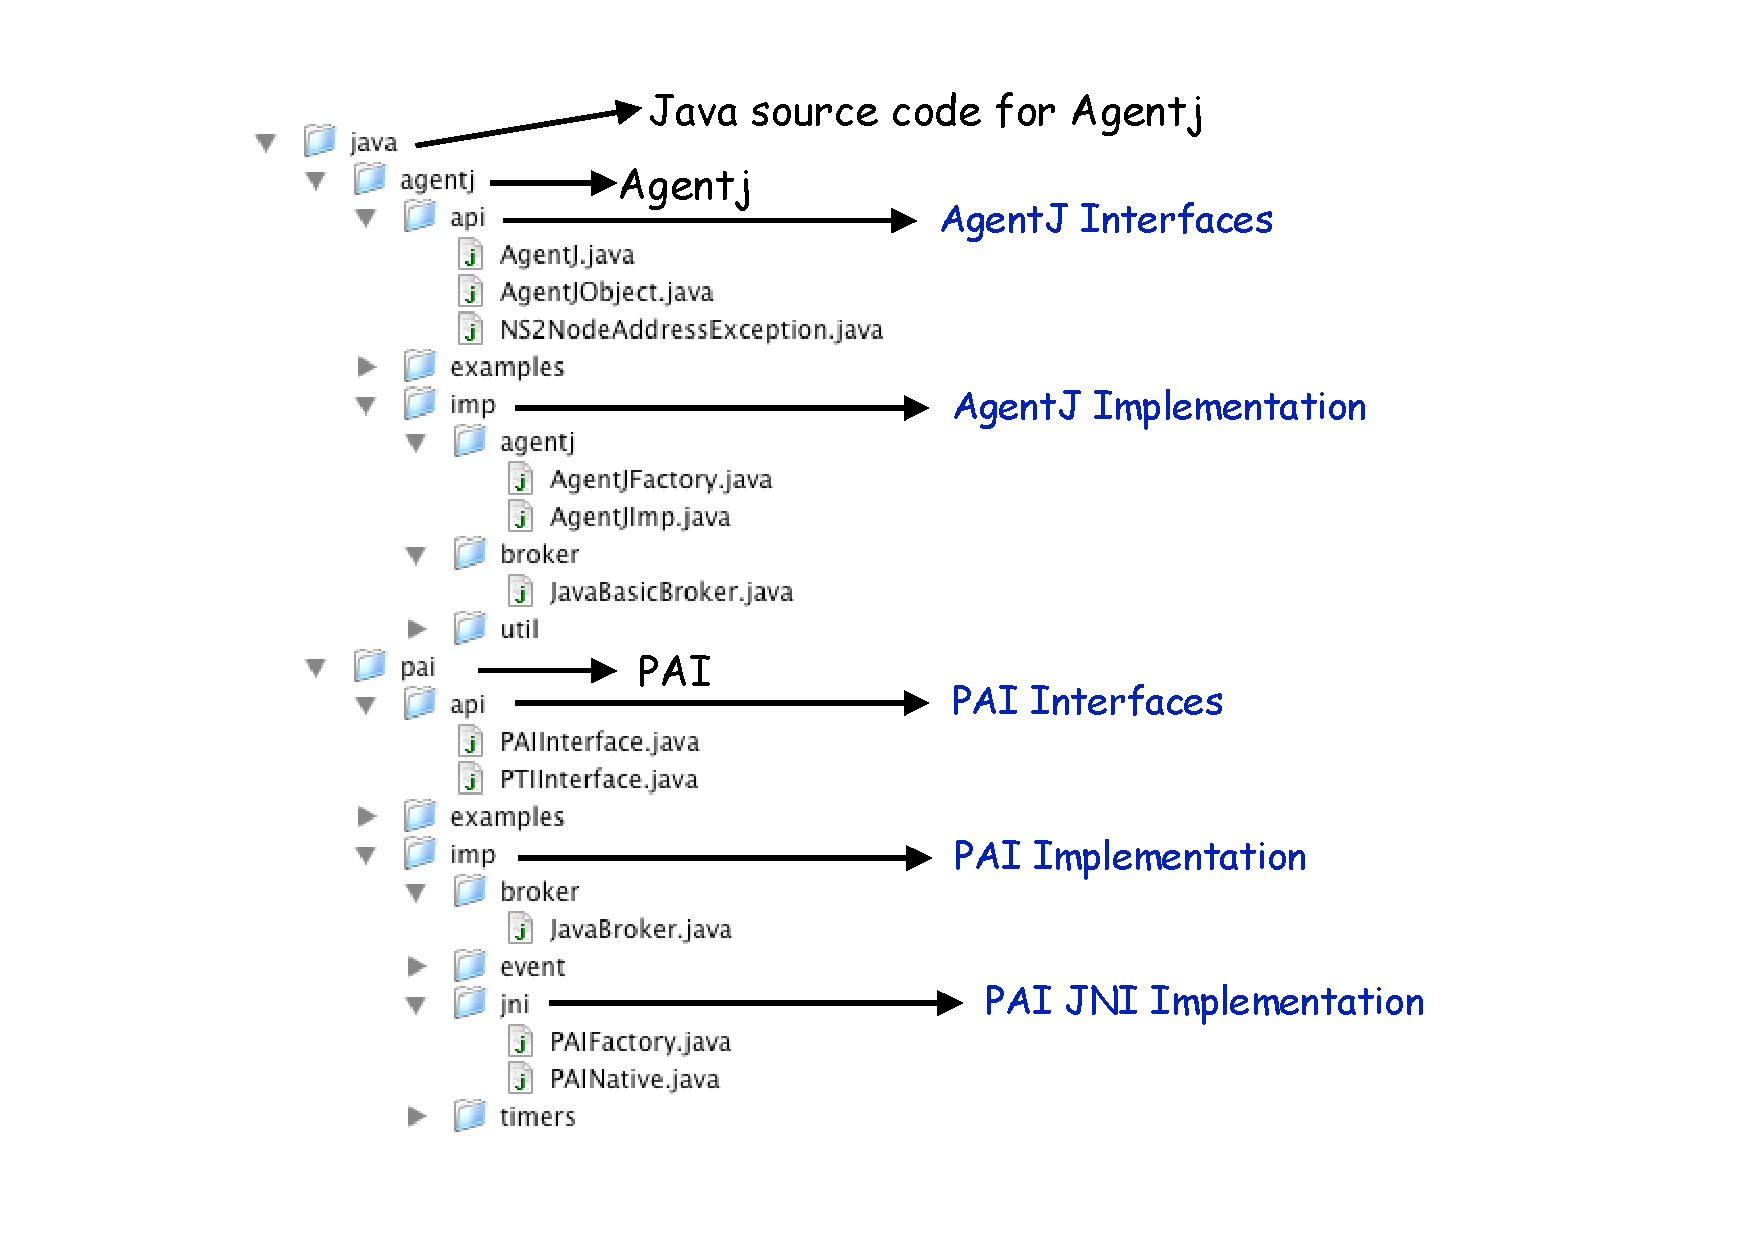
\includegraphics[scale=0.45]{images/agentjJavaClasses}
\caption{The Java Classes within \agentj.} 
\label{agentj:fig:JavaClasses}
\end{figure}


Beyond this, there are subdirectories that correspond to the
particular section of the overall implementation that those
classes are involved with. Therefore, theses directories are
organized as if they were Java packages (and indeed, in Java,
they ARE Java packages). Therefore, APIs (or Java interfaces 
to APIs) are always put in a directory called 'api' and 
implementations of such interfaces are always put in  
directories called 'imp'. Subsequently, implementations of different 
interfaces or APIs are inserted into different sub directories. 

These two Figures will be references in the next section, when we
discuss the specifics about the individual classes which are used
to implement parts of the overall system.
 
\subsection{Key \agentj~Classes}

The central class in \agentj, which implements the bridge between the 
C++ NS2  nodes and Java is \emph{Agentj.cpp} (found in  
\emph{Agentj/src/c/agentj}, see \ref{agentj:fig:CClasses}).  Agentj.cpp
inherits from Protolib's \emph{NsProtoAgent}, which
is a C++ NS2 agent, which can use the Protolib data transport 
implementation e.g. UDP and TCP, within NS2. \emph{Agentj} uses 
the \emph{Agentj} class to attach a Java Object to a C++ agent.  
Thereafter, the Java object itself interfaces through JNI to PAI, 
which in turn uses the Protolib to send the actual data packets. 

\begin{figure}
\centering
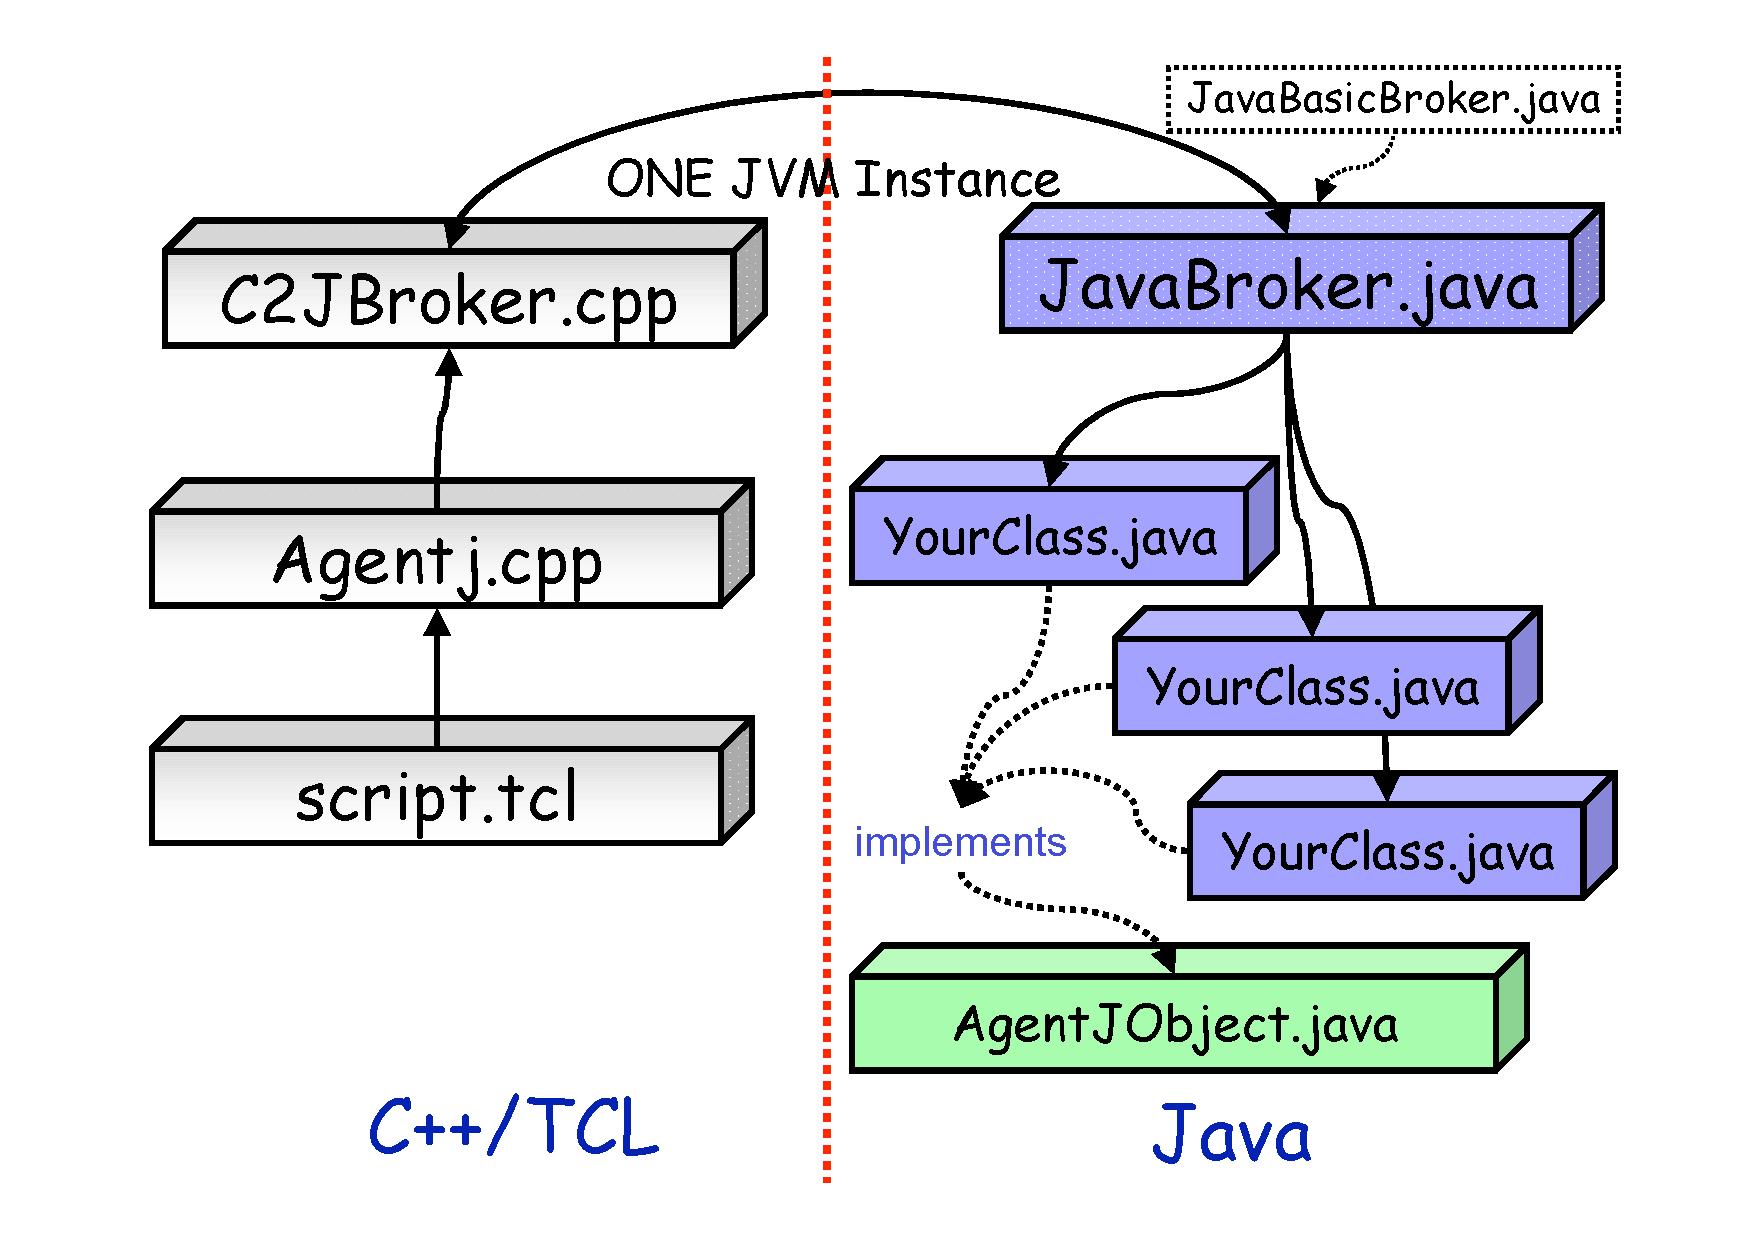
\includegraphics[scale=0.4]{images/agentjClasses}
\caption{The C++ and Java classes used to implement the TCL/C++ and Java
bridging mechanism.} 
\label{agentj:fig:jniClasses}
\end{figure}

As shown in Figure \ref{agentj:fig:jniClasses}, \emph{Agentj} uses the
C2JBroker C++ class to create a Java Virtual Machine (JVM) and 
communicate with the singleton \emph{JavaBroker} Java class.  
C2JBroker simply has these two functions:  it creates a JVM and 
provides a C++ interface for sending messages to the JavaBroker 
Java class. However, it also implements some finer grained 
functionality. C2JBroker initializes \agentj's environment variables.
It parses the LD\_LIBRARY\_PATH and CLASSPATH variables and
passes them to the JVM when it is being created so that the JVM
can use the standard initialization procedures.  It also, sets
up the debugging settings i.e. by checking the AGENTJDEBUG
and AGENTJXMLCONFIG variables (see Chapter \ref{install}).  


The \emph{JavaBroker} Java class allows provides a container 
for the Java objects that \agentj creates during the lifetime of the 
simulation.  A Java Hashtable is used to store each Java object 
along with its identifier, which is the reference to the NS2
agent that this Java object belongs to.  Each NS2 agent can
attach (instantiate) one Java class and therefore there is a 
one-to-one interaction between an NS2 agent and its Java object. 

These interactions are shown in detail in Figure \ref{agentj:fig:jniClasses}. 
Briefly, the programmer attaches the Java class within
the TCL script.  The JavaAgent then passes this data via \emph{C2JBroker}
to the \emph{JavaBroker} Java object. The \emph{JavaBroker} instantiates 
this object on-the-fly from the given class name.  This means that you can
attach multiple Java objects of the same type to every node or you are free
to attach different objects to different NS2 nodes, depending on what you 
want to implement.  For example, you could have a Java data collector 
agent talking to a Java data collection manager node instance. The only 
stipulation on the Java objects being created is that they should implement 
the \emph{AgentJObject} interface.
 
\begin{figure}
\centering
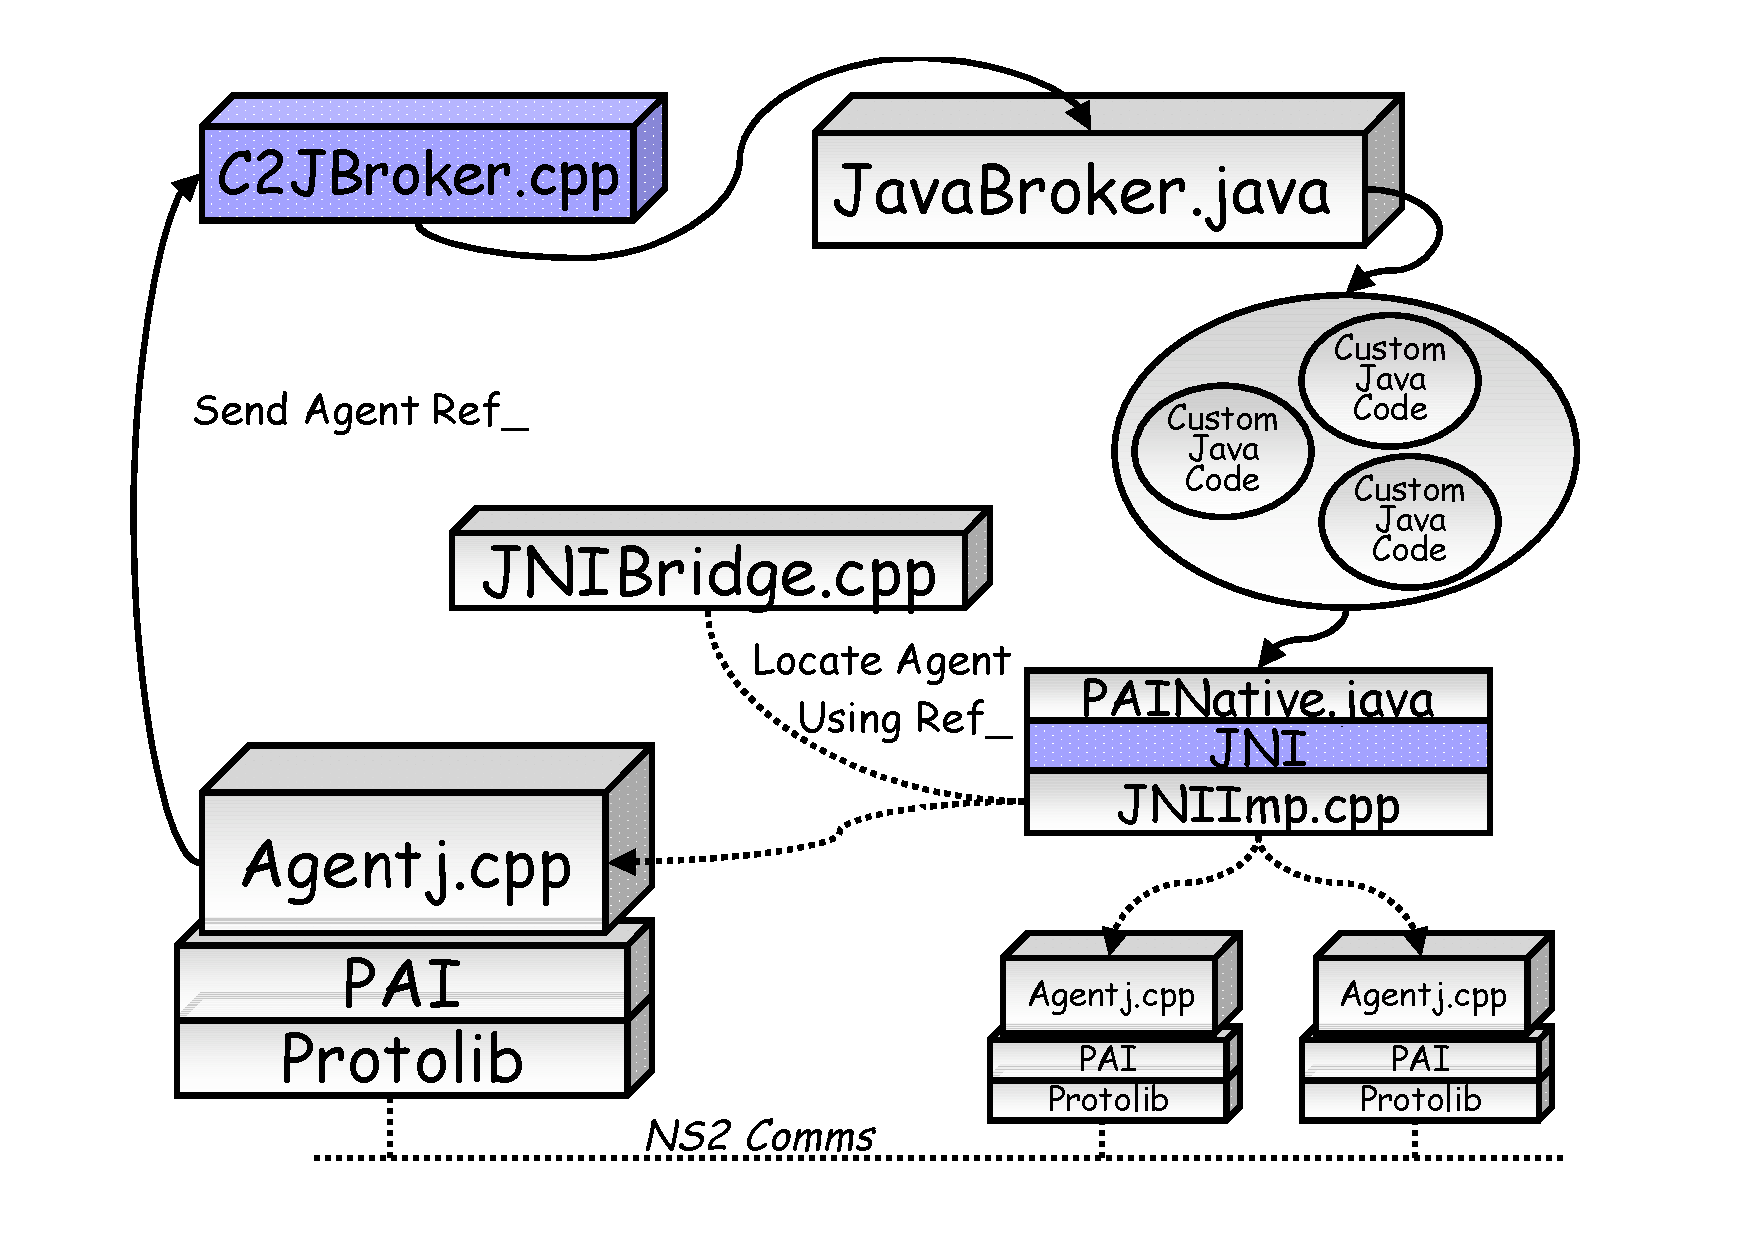
\includegraphics[scale=0.4]{images/agentjOverviewWithClasses}
\caption{The C++ and Java classes shown in the broad overview of \agentj.} 
\label{agentj:fig:agentjOverviewClasses}
\end{figure}


Figure \ref{agentj:fig:agentjOverviewClasses} shows the \agentj architecture
given in Figure \ref{agentj:fig:javaFullOverview} but inserts the various C++ and
Java classes which are used to implement each of the interactions. This clearly illustrates the interaction between
the \emph{Agentj}, \emph{C2JBroker} and \emph{JavaBroker} 
classes. Notice here that also the purpose of the \emph{JavaBroker}
is also illustrated; that is, it acts as a container for the multiple Java
objects (\agentj~nodes) that \agentj~creates. 

Also, depicted here, are the classes involved in the Java and JNI 
implementation of the PAI interface.  The Java PAI interface is outline in 
the next subsection and is implemented by the \emph{PAINative} Java 
class, which binds this interface, through JNI to the underlying C++ 
PAI implementation.  Within this implementation, there are two key 
C++ classes: \emph{JNIImp} and \emph{JNIBridge}. JNIImp is
a direct implementation of the Java native methods contained within
the PAINative Java class, whilst \emph{JNIBridge} provides a 
persistent C++ object for storing information about the state of the
C++ PAI interface during this session.  

For example, \emph{JNIBridge}
contains the list of Java to C++ mappings of the various listeners that
have been attached to the numerous sockets and timers which may
have been created by the Java application.  It also implements the
callbacks to Java, which in turn, result in an event being passed 
to the Java classes which have requested to be notified about 
such events. This is a somewhat complicated procedure because
C++ callbacks to Java have no context, so they must invoke a static
Java method using an identifier notifying it which socket or timer
this event belongs to. From this information, the Java method can
work out which listeners are interested in this event.   


\subsection{The Java PAI interface}
\label{jnipai:jpai}

The Java PAI implementation consists of two Java interfaces:

\begin{itemize}
\item \textbf{PAIInterface:}  interfaces to the communication part of the 
PAI interface (i.e. the sockets).  
\item \textbf{PTIInterface:}  interfaces to the timing part of the 
PAI interface (i.e. the timers).  
\end{itemize}

 
The \emph{PAIInterface} allows the user to create multiple sockets and 
allows multiple socket listeners to be attached to each socket.  This 
functionality is necessary for Java applications and
is illustrated in the P2PS implementation, described in \cite{p2psx}.
The \emph{PTIInterface} does the same for timers.  However,
it is \textbf{important to note} that a user of \agentj does not have
to use these classes directly. In fact, a user should not use these 
classes directly!  They should use the PAI implementations
of the UDP, TCP and timing interfaces for the default Java 
interfaces to these classes e.g. if you want to create a UDP
socket then you should create a \emph{pai.net.DatagramSocket},
which behaves exactly the same as a 
\emph{java.net.DatagramSocket} except that it works within NS2.
The interfaces here merely describe the lower level interfaces and
mechanisms that are used to implement the overall structure.

The Java PAI interface is defined using a collection of Java 
interfaces and uses the \emph{Factory Method Design} pattern 
\cite{designpatterns} in order to create the appropriate underlying
implementation.  This means that other implementations (e.g. a native
Java implementation) could be implemented at a later date.
The application developer however, would not notice this code
change because s/he is working with a consistent interface.  The
JPAI interface can be found in package \emph{pai.api} in the
Java source tree and is listed below:

\footnotesize
\begin{verbatim}

public interface PAIInterface extends PTIInterface {
    void init();
    
    void addPAISocketListener(DatagramSocket sock, PAISocketListener listener);

    void removePAISocketListener(DatagramSocket sock, PAISocketListener listener);

    void open(DatagramSocket sock, int port) throws SocketException;

    DatagramSocket addSocket(int port) throws SocketException;

    void removeSocket(DatagramSocket sock) throws SocketException;

    void setReuseAddress(DatagramSocket sock, boolean on) throws SocketException;

    void setSendBufferSize(DatagramSocket sock, int size) throws SocketException;

    void setReceiveBufferSize(DatagramSocket sock, int size) throws SocketException;

    void setSoTimeout(DatagramSocket sock, int timeout) throws SocketException;

    void send(DatagramSocket sock, DatagramPacket p) throws IOException;

    void receive(DatagramSocket sock, DatagramPacket p) throws IOException;

    void close(DatagramSocket sock);

    void joinGroup(MulticastSocket sock, InetAddress mcastaddr) throws IOException;

    void leaveGroup(MulticastSocket sock, InetAddress mcastaddr) throws IOException;

    void setMulticast(MulticastSocket sock, boolean val);

    public InetAddress getByName(String host) throws UnknownHostException;

    public InetAddress getLocalHost();

    public boolean cleanUp();
    public boolean runBlock();
    public boolean runNonBlock();

    public void setNS2Node(String nodeID);

    public void setNS2Scheduler(String schedulerID);
}
\end{verbatim}
\normalsize
  
Most of the calls are self-explanatory.  PAI uses the Java conventions
for naming the classes e.g. DatagramSocket and MulticastSocket, both found
in the java.net package (see \cite{javaTutorial}). The PAI Java 
implementation reimplements the methods from these classes in order
to use the PAI interface.  This enables the PAI interface to provide the 
functionality but it leaves the Java interface that developers are familiar
with the same. Therefore, to create a Java UDP socket, you simply
instantiate a DatagramSocket, which in turn invokes PAI to create
a C++ PAI socket, which in turn creates a Protolib socket.   

The \emph{PTIInterface} is much simpler:

\footnotesize
\begin{verbatim}

public interface PTIInterface {
    PAITimer addTimer(double delay, int repeat);

    void removeTimer(PAITimer timer);

    void addPAITimerListener(PAITimer timerID, PAITimerListener listener);

    void removePAITimerListener(PAITimer timerID, PAITimerListener listener);

    boolean runTimers();
}

\end{verbatim}
\normalsize

Here, we simply provide a mechanism for creating a simple timer and
allow a Java application to attach multiple listeners to it.
 
This design carries the whole weight of the \agentj implementation.  
To an application, the use of the conventional Java interface for 
creating  UDP sockets means that they require very 
little source code modification in order to use this PAI JNI binding here.
For example, in order to get P2PS working (see \cite{p2psx}) with this 
interface, a new resolver was created for UDP. This was a direct copy 
of the Java UDP resolver code with the occurrences of \emph{java.net} 
replaced with \emph{pa.net}, which enables this new resolver to look in
the appropriateplace for the PAI DatagramSocket class. Everything else 
followed through the various layers and P2PS required no further 
modification at the transport level. This re-implementation of these base 
Java classes can be found in the \emph{pai.net} package in the source tree. 

\section{Conclusion}

In this chapter, an overview of the \agentj~integration was given, from
a conceptual perspective and a source-code perspective. We illustrated
the design and architecture of \agentj~then described in detail the
interaction between the C++ and Java sections of the system.  We then
delved into the Java and C++ classes and outlined the key classes
that implement this functionality and further, outlined the directory structure
for \agentj~ for reference.  We then inserted the names of these classes
back into the architectural overview to give a clear picture of the entire
system and the key components thereof.  Finally, we gave a brief
outline of the Java PAI interface to illustrate the kind of functionality it
provides.
  


